\section{Muhammad Afra Faris/1174041}
\subsection{Soal 1}
Fungsi, Sejarah, dan Contoh file CSV : 
\begin{itemize}
	\item Fungsi : 
	File Comma Separated Values atau  biasa disingkat dengan CSV merupakan tipe file khusus yang menyimpan informasi dengan metode dipisahkan dengan koma. File CSV berfungsi untuk menjadi perantara beberapa aplikasi yang memiliki basis data saat pengiriman data. CSV juga dapat dibuka di berbagai text editor. Dengan bentuk filenya yang dinamis, file CSV mungkin dapat dimanipulasi dan dapat menyimpan informasi dengan skala besar.
	\item Sejarah :
	CSV ini sudah digunakan sejak tahun 1972 yang dapat dikompilasi pada bahasa pemrograman IBM Fortran. Pada saat itu, data yang dipisahkan oleh koma jika isinya memiliki spasi maka harus diberi tanda petik di awal dan akhir isi dari data tersebut. Nama CSV ini baru mulai digunakan pada tahun 1983. Pada panduan dari Osborne Executive Computer mendokumentasikan kutipan yang membolehkan isi karakter memiliki koma.  Tahun 2005 dengan RFC4180, CSV didefinisikan sebagai MIME Content Type. lalu pada tahun 2013, defisiensi dari RFC4180 dipecahkan oleh rekomendasi dari W3C. Tahun 2014, IETF mempublikasi RFC7111 yang mendeskripsikan pecahan Uniform Resource Identifier(URI) ke dokumen CSV. RFC7111 menjelaskan bagaimana baris, kolom dapat dipilih dalam dokumen CSV menggunakan indeks posisi. Pada Tahun 2015,  draft rekomendasi untuk CSV-metadata standards dipublikasikan W3C yang dimulai dengan rekomendasi pada bulan Desember dengan tahun yang sama. 
	\item Contoh File CSV \begin{itemize}
							\item 
							CSV pada Excel \ref{csvex}
							\begin{figure}[!htbp]
								\centering
								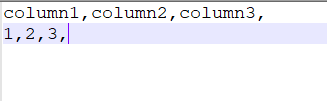
\includegraphics[height=4cm, width=7cm]{figures/4/1174041/Teori/csvex.png}
								\caption{Contoh CSV Pada Excel}
								\label{csvex}
							\end{figure}
														
						  \end{itemize}
\end{itemize}
\subsection{Soal 2}
Aplikasi Yang dapat membuat file CSV : 
Berikut file yang dapat membuat file CSV
\begin{itemize}
	\item Spreadsheet :
	Spreadsheet adalah aplikasi yang bisa digunakan membuat CSV hanya dengan memasukan data sesuai baris dan kolom yang diinginkan. Contoh dari spreadsheet seperti Microsoft Excel, Google Spreadsheet, dan beberapa aplikasi lainnya. 
	\item Bahasa Pemrograman :
	Bahasa pemrograman adalah sarana media yang dapat digunakan untuk membuat aplikasi, yang bisa membuat file CSV khusus untuk bahasa pemrograman yang mendukung dengan pembuatan file CSV. Seperti Python, C Sharp, dan lain sebagainya.
	\item Text Editor :
	Text editor juga dapat digunakan untuk membuat file CSV. Untuk membuat file CSV dengan Text Editor cukup dengan membuat file sesuai format CSV dan save file tersebut dengan ekstensi .CSV.
\end{itemize}
\subsection{Soal 3}
Menulis dan Membaca file CSV : 
Berikut cara menulis dan membaca file CSV : 
\begin{itemize}
	\item Menulis : \begin{enumerate}
						\item Buka file CSV dengan spreadsheet apapun
						\item Klik Cell yang akan dimasukkan
						\item Masukan data yang akan dimasukkan pada cell tersebut
						\item Lalu save file dengan format .CSV
					\end{enumerate}
	\item Membaca : \begin{enumerate}
						\item Buka file CSV dengan spreadsheet						
					\end{enumerate}
\end{itemize}
\subsection{Soal 4}
Sejarah Library CSV Python : 
Library CSV pada python merupakan library yang paling umum untuk import export data pada spreadsheet dan basis data dengan format sesuai dengan standarisasi RFC4180. Seiring dengan lahirnya bahasa pemrograman python, library mulai dibuat dan dikembangkan sampai akhirnya pada tahun 2003, pembuatnya Kevin Altis dan lainnya telah merilis versi final untuk library Python CSV. 
\subsection{Soal 5}
Sejarah Library Pandas Python : 
Pandas (Python Data Analysis Library) adalah library open source yang digunakan untuk melakukan data manajemen dan data analysis. Pandas diciptakan pada tahun 2008 oleh Wes McKinney dan diperbaharui oleh Sien Chang pada tahun 2010. Inspirasi dari pembuatan pandas muncul pada komunitas yang membutuhkan library khusus untuk analisis data. 
\subsection{Soal 6}
Fungsi - fungsi yang terdapat di library CSV : 
\begin{itemize}
	\item \begin{verbatim} csv.reader(csvfile, dialect='excel', **fmtparams) \end{verbatim} Untuk mengembalikan	object reader yang akan mengambil setiap line pada csv yang diambil. Data setiap baris diambil saat next() dipanggil. 
	\item \begin{verbatim} csv.writer(csvfile, dialect='excel', **fmtparams) \end{verbatim} Mengembalikan file pembuat object untuk dapat mengkonversi data pada python ke file CSV yang akan dibuat. 
	\item \begin{verbatim} csv.register_dialect(name[, dialect[, **fmtparams]]) \end{verbatim} Mengasosiasikan dialek dengan nama, dan nama yang dimasukkan harus berupa karakter.
	\item \begin{verbatim} csv.unregister_dialect(name) \end{verbatim}
	Menghapus asosiasi dialek dengan nama yang ada pada registry dialek.
	\item \begin{verbatim} csv.get_dialect(name) \end{verbatim}
	Mengambil dialek yang telah diasosiasikan dengan nama. 
	\item \begin{verbatim}  csv.list_dialects() \end{verbatim} Mengembalikan dialek yang telah terregistrasi.
	\item \begin{verbatim} csv.field_size_limit([new_limit]) \end{verbatim} Mengembalikan maksimal column data yang diperbolehkan oleh pembaca.
\end{itemize}
\subsection{Soal 7}
Fungsi - fungsi yang terdapat di library Pandas : 
\begin{itemize}
	\item \begin{verbatim} pandas.read_excel(io[, sheet_name, header, names, …])  \end{verbatim} Membaca file excel dan menyimpan ke DataFrame.
	\item \begin{verbatim} pandas.read_csv(filepath_or_buffer[, sep, …]) \end{verbatim} Untuk membaca file CSV dan menyimpan ke DataFrame.
	\item \begin{verbatim} to_csv([path, index, sep, na_rep, …]) \end{verbatim}
	Untuk membuat file CSV dari data yang telah ada.	
\end{itemize}
\subsection{Cek Plagiarism}
Berikut pengecekan plagiarism yang dilakukan pada website smallseotools.com : 
\begin{figure}[!htbp]
	\centering
	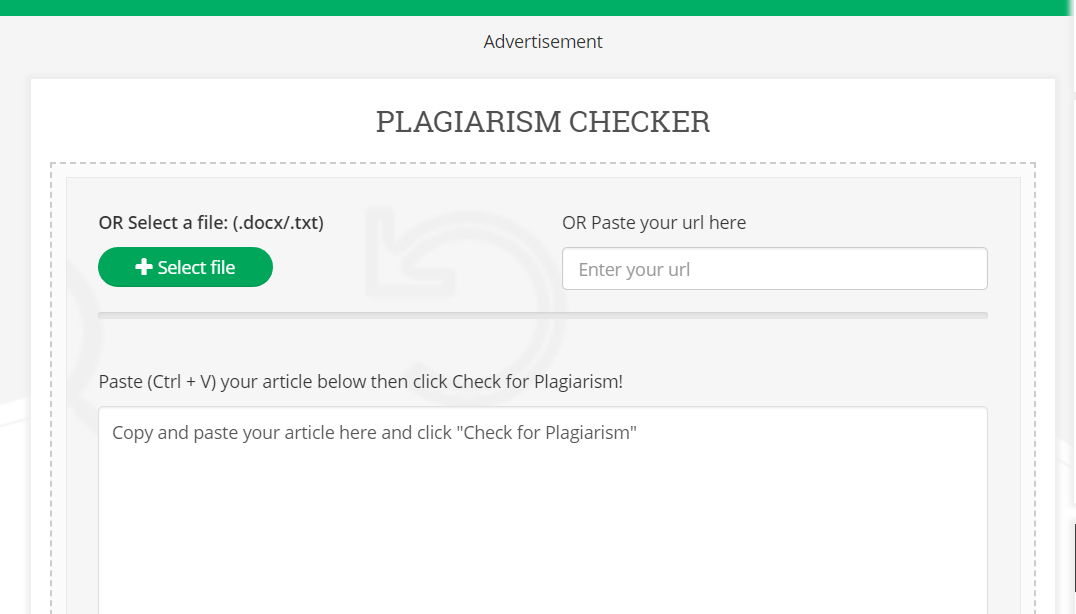
\includegraphics[height=6cm, width=10cm]{figures/4/1174041/Teori/plagiarism.png}
	\caption{Cek Plagiarisme}
	\label{plagiarism}
\end{figure}